\section{Referencia de la Clase Inventario}
\label{classInventario}\index{Inventario@{Inventario}}
Administra los datos de inventario.  


{\tt \#include $<$inventario.h$>$}

Diagrama de herencias de Inventario\begin{figure}[H]
\begin{center}
\leavevmode
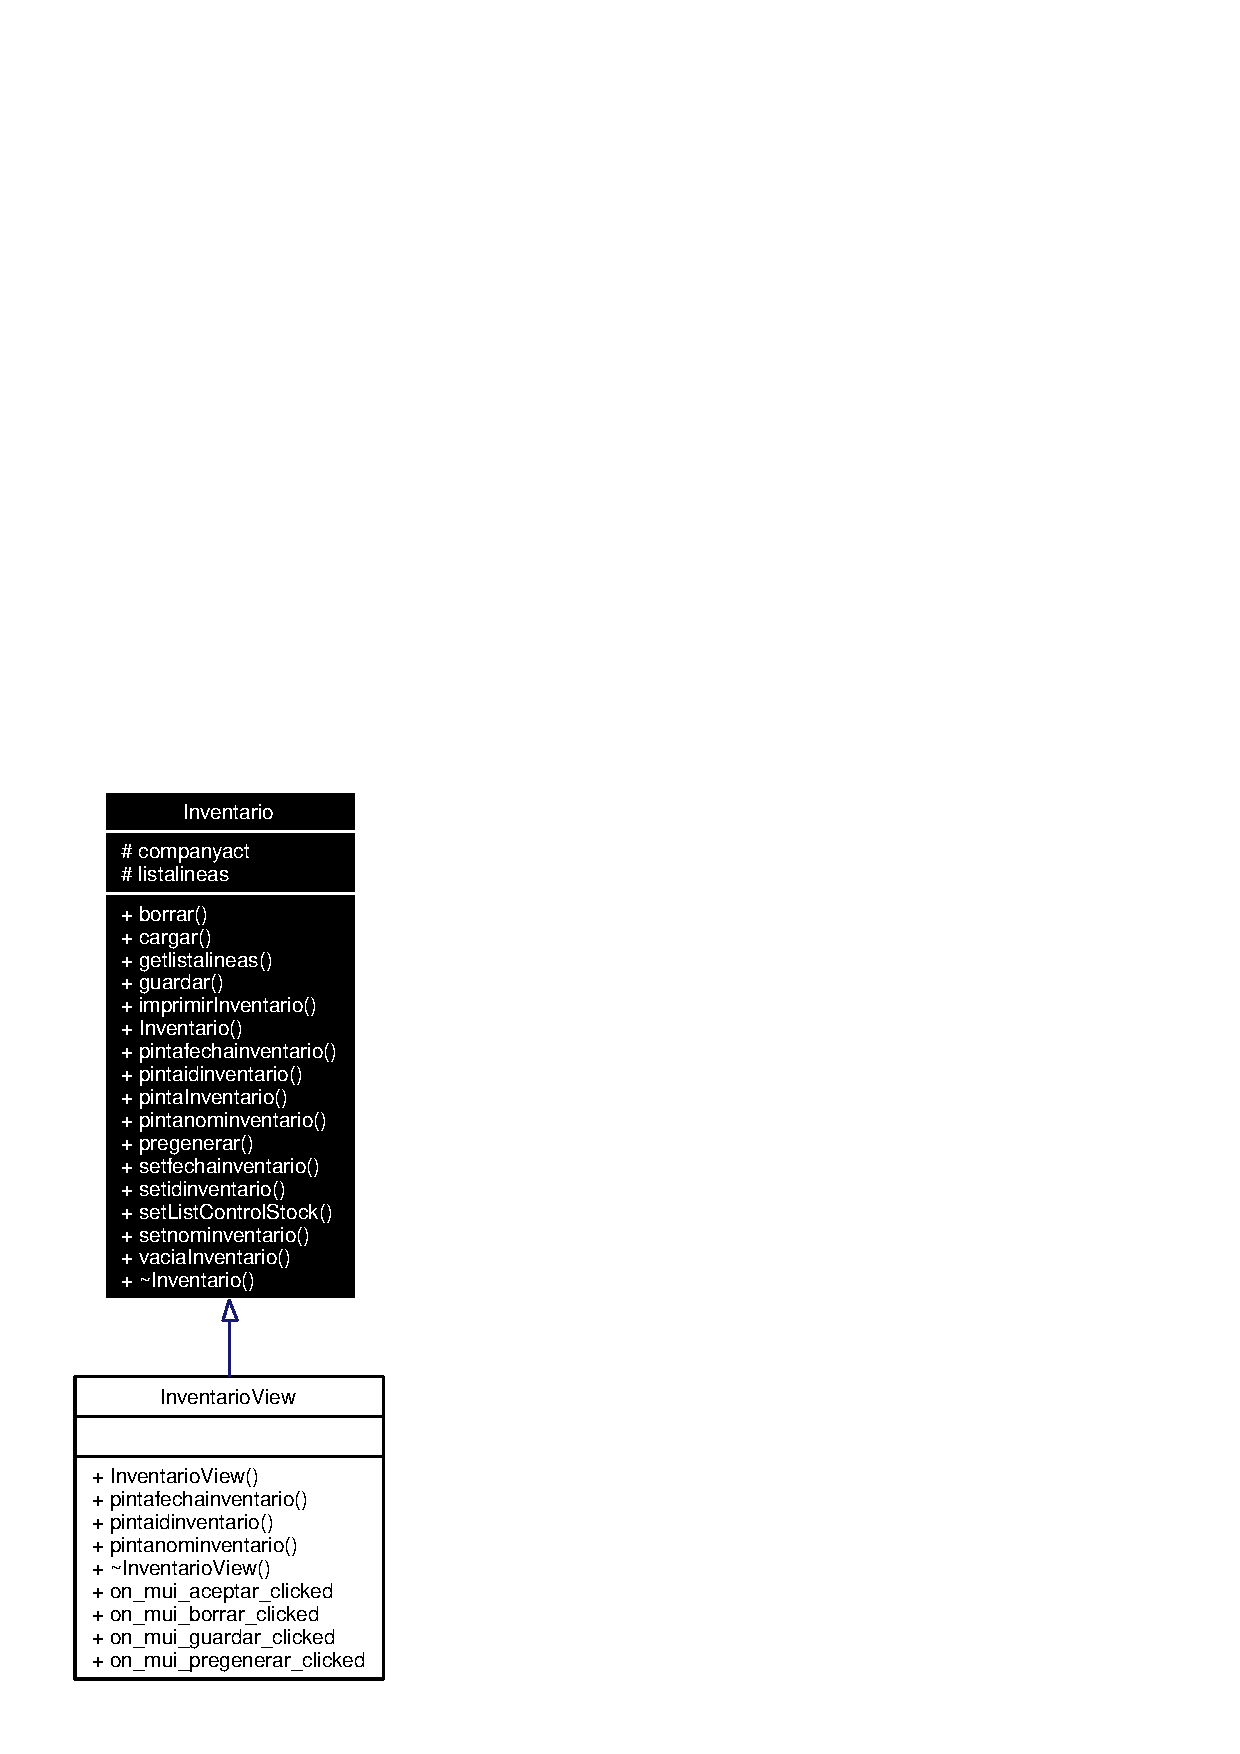
\includegraphics[width=92pt]{classInventario__inherit__graph}
\end{center}
\end{figure}
Diagrama de colaboraci\'{o}n para Inventario:\begin{figure}[H]
\begin{center}
\leavevmode
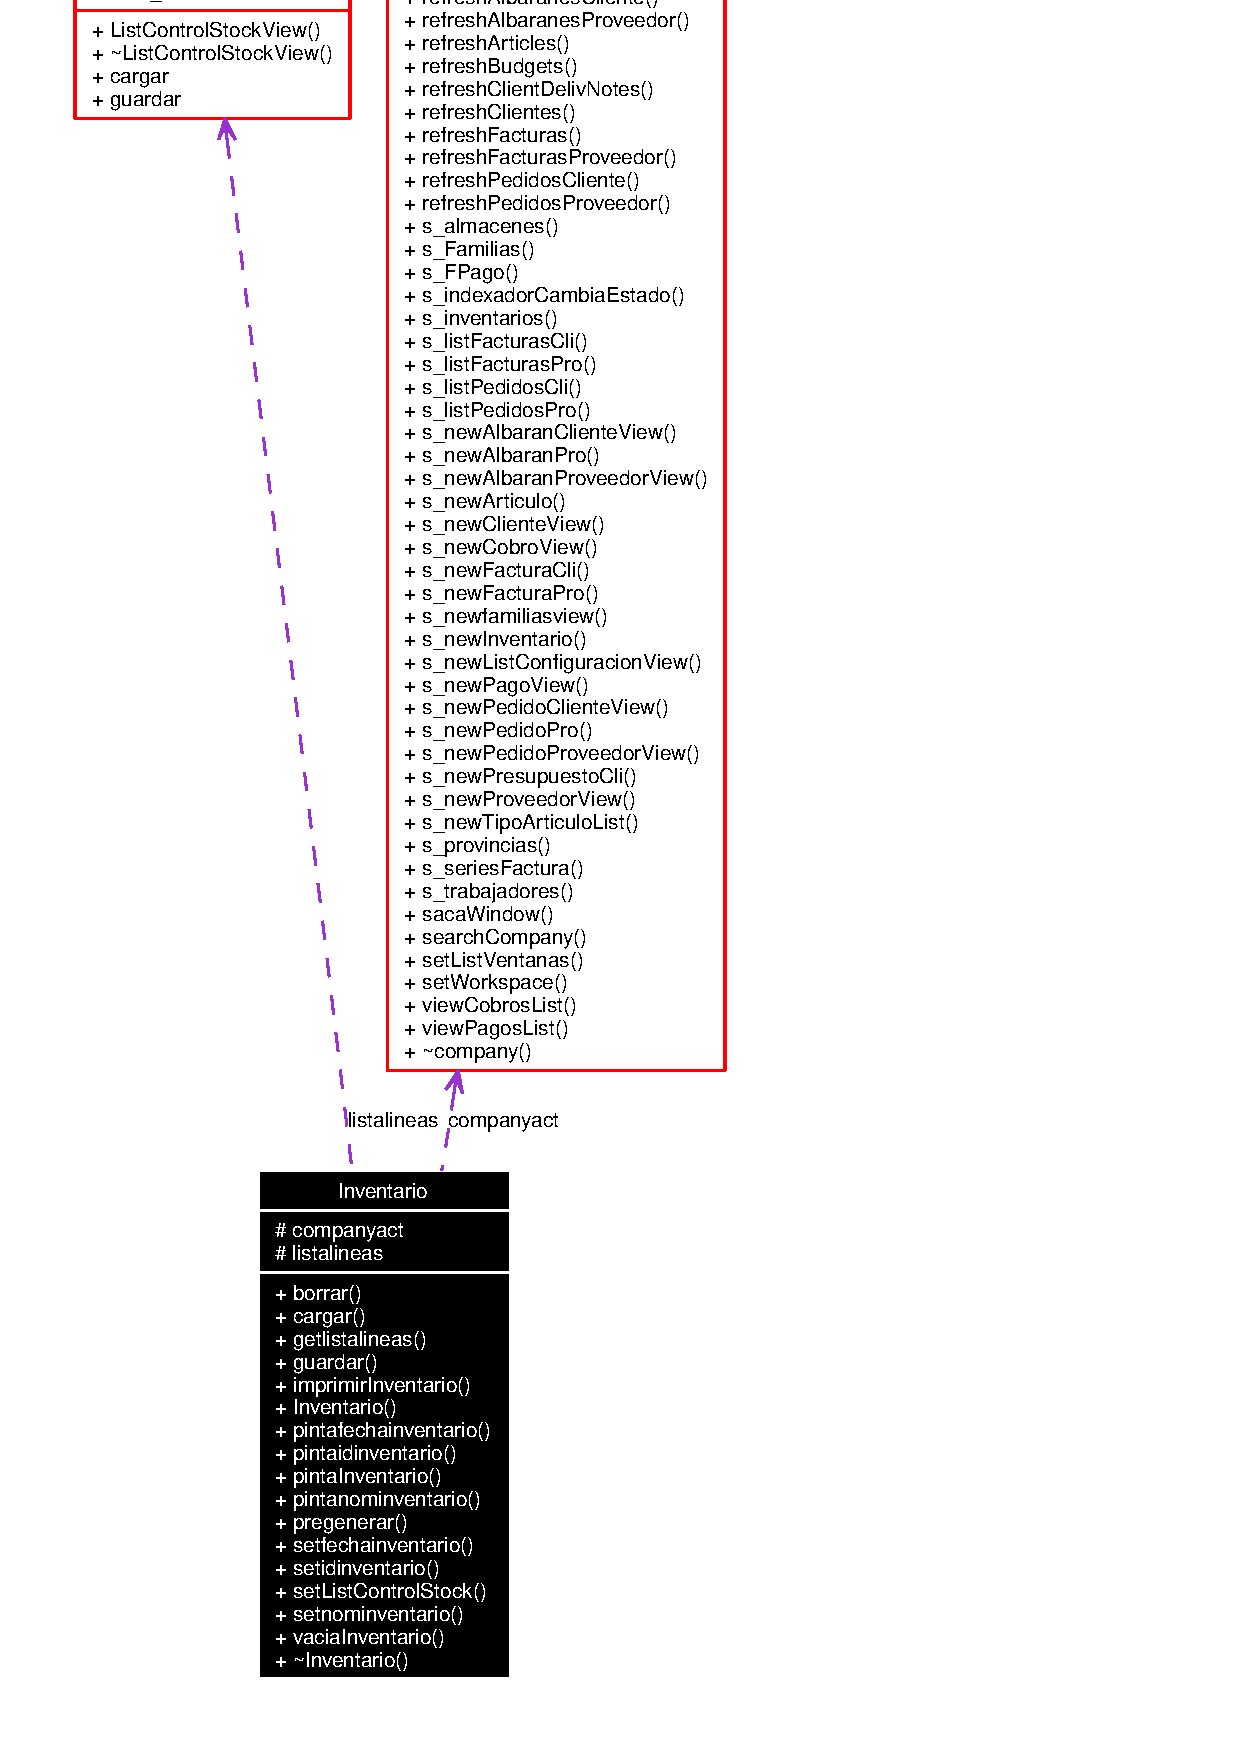
\includegraphics[width=174pt]{classInventario__coll__graph}
\end{center}
\end{figure}
\subsection*{M\'{e}todos p\'{u}blicos}
\begin{CompactItemize}
\item 
virtual int {\bf borrar} ()\label{classInventario_a0}

\item 
virtual int {\bf cargar} (QString)\label{classInventario_a1}

\begin{CompactList}\small\item\em Esta funcion carga un Inventario. \item\end{CompactList}\item 
{\bf List\-Control\-Stock\-View} $\ast$ {\bf getlistalineas} ()\label{classInventario_a2}

\item 
virtual int {\bf guardar} ()\label{classInventario_a3}

\item 
void {\bf imprimir\-Inventario} ()\label{classInventario_a4}

\item 
{\bf Inventario} ({\bf company} $\ast$)\label{classInventario_a5}

\item 
virtual void {\bf pintafechainventario} (QString)\label{classInventario_a6}

\item 
virtual void {\bf pintaidinventario} (QString)\label{classInventario_a7}

\item 
void {\bf pinta\-Inventario} ()
\item 
virtual void {\bf pintanominventario} (QString)\label{classInventario_a9}

\item 
virtual void {\bf pregenerar} ()\label{classInventario_a10}

\item 
void {\bf setfechainventario} (QString val)\label{classInventario_a11}

\item 
void {\bf setidinventario} (QString val)\label{classInventario_a12}

\item 
void {\bf set\-List\-Control\-Stock} ({\bf List\-Control\-Stock\-View} $\ast$a)\label{classInventario_a13}

\item 
void {\bf setnominventario} (QString val)\label{classInventario_a14}

\item 
void {\bf vacia\-Inventario} ()\label{classInventario_a15}

\end{CompactItemize}
\subsection*{Atributos protegidos}
\begin{CompactItemize}
\item 
{\bf company} $\ast$ {\bf companyact}\label{classInventario_p0}

\item 
{\bf List\-Control\-Stock\-View} $\ast$ {\bf listalineas}\label{classInventario_p1}

\end{CompactItemize}


\subsection{Descripci\'{o}n detallada}
Administra los datos de inventario. 



\subsection{Documentaci\'{o}n de las funciones miembro}
\index{Inventario@{Inventario}!pintaInventario@{pintaInventario}}
\index{pintaInventario@{pintaInventario}!Inventario@{Inventario}}
\subsubsection{\setlength{\rightskip}{0pt plus 5cm}void Inventario::pinta\-Inventario ()}\label{classInventario_a8}


Pinta el subformulario de detalle del Inventario. 

La documentaci\'{o}n para esta clase fu\'{e} generada a partir de los siguientes archivos:\begin{CompactItemize}
\item 
inventario.h\item 
inventario.cpp\end{CompactItemize}
